% Options for packages loaded elsewhere
\PassOptionsToPackage{unicode}{hyperref}
\PassOptionsToPackage{hyphens}{url}
%
\documentclass[
]{article}
\usepackage{lmodern}
\usepackage{amssymb,amsmath}
\usepackage{ifxetex,ifluatex}
\ifnum 0\ifxetex 1\fi\ifluatex 1\fi=0 % if pdftex
  \usepackage[T1]{fontenc}
  \usepackage[utf8]{inputenc}
  \usepackage{textcomp} % provide euro and other symbols
\else % if luatex or xetex
  \usepackage{unicode-math}
  \defaultfontfeatures{Scale=MatchLowercase}
  \defaultfontfeatures[\rmfamily]{Ligatures=TeX,Scale=1}
\fi
% Use upquote if available, for straight quotes in verbatim environments
\IfFileExists{upquote.sty}{\usepackage{upquote}}{}
\IfFileExists{microtype.sty}{% use microtype if available
  \usepackage[]{microtype}
  \UseMicrotypeSet[protrusion]{basicmath} % disable protrusion for tt fonts
}{}
\makeatletter
\@ifundefined{KOMAClassName}{% if non-KOMA class
  \IfFileExists{parskip.sty}{%
    \usepackage{parskip}
  }{% else
    \setlength{\parindent}{0pt}
    \setlength{\parskip}{6pt plus 2pt minus 1pt}}
}{% if KOMA class
  \KOMAoptions{parskip=half}}
\makeatother
\usepackage{xcolor}
\IfFileExists{xurl.sty}{\usepackage{xurl}}{} % add URL line breaks if available
\IfFileExists{bookmark.sty}{\usepackage{bookmark}}{\usepackage{hyperref}}
\hypersetup{
  pdftitle={Phenology in R},
  pdfauthor={Atkins, Stovall, and Silva},
  hidelinks,
  pdfcreator={LaTeX via pandoc}}
\urlstyle{same} % disable monospaced font for URLs
\usepackage[margin=1in]{geometry}
\usepackage{color}
\usepackage{fancyvrb}
\newcommand{\VerbBar}{|}
\newcommand{\VERB}{\Verb[commandchars=\\\{\}]}
\DefineVerbatimEnvironment{Highlighting}{Verbatim}{commandchars=\\\{\}}
% Add ',fontsize=\small' for more characters per line
\usepackage{framed}
\definecolor{shadecolor}{RGB}{248,248,248}
\newenvironment{Shaded}{\begin{snugshade}}{\end{snugshade}}
\newcommand{\AlertTok}[1]{\textcolor[rgb]{0.94,0.16,0.16}{#1}}
\newcommand{\AnnotationTok}[1]{\textcolor[rgb]{0.56,0.35,0.01}{\textbf{\textit{#1}}}}
\newcommand{\AttributeTok}[1]{\textcolor[rgb]{0.77,0.63,0.00}{#1}}
\newcommand{\BaseNTok}[1]{\textcolor[rgb]{0.00,0.00,0.81}{#1}}
\newcommand{\BuiltInTok}[1]{#1}
\newcommand{\CharTok}[1]{\textcolor[rgb]{0.31,0.60,0.02}{#1}}
\newcommand{\CommentTok}[1]{\textcolor[rgb]{0.56,0.35,0.01}{\textit{#1}}}
\newcommand{\CommentVarTok}[1]{\textcolor[rgb]{0.56,0.35,0.01}{\textbf{\textit{#1}}}}
\newcommand{\ConstantTok}[1]{\textcolor[rgb]{0.00,0.00,0.00}{#1}}
\newcommand{\ControlFlowTok}[1]{\textcolor[rgb]{0.13,0.29,0.53}{\textbf{#1}}}
\newcommand{\DataTypeTok}[1]{\textcolor[rgb]{0.13,0.29,0.53}{#1}}
\newcommand{\DecValTok}[1]{\textcolor[rgb]{0.00,0.00,0.81}{#1}}
\newcommand{\DocumentationTok}[1]{\textcolor[rgb]{0.56,0.35,0.01}{\textbf{\textit{#1}}}}
\newcommand{\ErrorTok}[1]{\textcolor[rgb]{0.64,0.00,0.00}{\textbf{#1}}}
\newcommand{\ExtensionTok}[1]{#1}
\newcommand{\FloatTok}[1]{\textcolor[rgb]{0.00,0.00,0.81}{#1}}
\newcommand{\FunctionTok}[1]{\textcolor[rgb]{0.00,0.00,0.00}{#1}}
\newcommand{\ImportTok}[1]{#1}
\newcommand{\InformationTok}[1]{\textcolor[rgb]{0.56,0.35,0.01}{\textbf{\textit{#1}}}}
\newcommand{\KeywordTok}[1]{\textcolor[rgb]{0.13,0.29,0.53}{\textbf{#1}}}
\newcommand{\NormalTok}[1]{#1}
\newcommand{\OperatorTok}[1]{\textcolor[rgb]{0.81,0.36,0.00}{\textbf{#1}}}
\newcommand{\OtherTok}[1]{\textcolor[rgb]{0.56,0.35,0.01}{#1}}
\newcommand{\PreprocessorTok}[1]{\textcolor[rgb]{0.56,0.35,0.01}{\textit{#1}}}
\newcommand{\RegionMarkerTok}[1]{#1}
\newcommand{\SpecialCharTok}[1]{\textcolor[rgb]{0.00,0.00,0.00}{#1}}
\newcommand{\SpecialStringTok}[1]{\textcolor[rgb]{0.31,0.60,0.02}{#1}}
\newcommand{\StringTok}[1]{\textcolor[rgb]{0.31,0.60,0.02}{#1}}
\newcommand{\VariableTok}[1]{\textcolor[rgb]{0.00,0.00,0.00}{#1}}
\newcommand{\VerbatimStringTok}[1]{\textcolor[rgb]{0.31,0.60,0.02}{#1}}
\newcommand{\WarningTok}[1]{\textcolor[rgb]{0.56,0.35,0.01}{\textbf{\textit{#1}}}}
\usepackage{graphicx}
\makeatletter
\def\maxwidth{\ifdim\Gin@nat@width>\linewidth\linewidth\else\Gin@nat@width\fi}
\def\maxheight{\ifdim\Gin@nat@height>\textheight\textheight\else\Gin@nat@height\fi}
\makeatother
% Scale images if necessary, so that they will not overflow the page
% margins by default, and it is still possible to overwrite the defaults
% using explicit options in \includegraphics[width, height, ...]{}
\setkeys{Gin}{width=\maxwidth,height=\maxheight,keepaspectratio}
% Set default figure placement to htbp
\makeatletter
\def\fps@figure{htbp}
\makeatother
\setlength{\emergencystretch}{3em} % prevent overfull lines
\providecommand{\tightlist}{%
  \setlength{\itemsep}{0pt}\setlength{\parskip}{0pt}}
\setcounter{secnumdepth}{-\maxdimen} % remove section numbering

\title{Phenology in R}
\author{Atkins, Stovall, and Silva}
\date{5/11/2020}

\begin{document}
\maketitle

\hypertarget{phenology-in-r-with-phenocamr}{%
\subsection{Phenology in R with
phenocamr}\label{phenology-in-r-with-phenocamr}}

\texttt{phenocamr} version 1.1.4 is availble on CRAN
\url{https://cran.r-project.org/web/packages/phenocamr/index.html} with
a development version availble on GitHUB
\url{https://github.com/khufkens/phenocamr}. A more in-depth tutorial is
availble via the National Ecological Observatory Network's (NEON) Data
Tutorial Series
\url{https://www.neonscience.org/phenocam-phenor-modeling}. Note, this
tutorial also includes information on additional data packages,
including some not availble currently on CRAN.

Here we show how to analyze phenocam data, taken from the PhenoCAM
network \url{https://phenocam.sr.unh.edu/webcam/} for the \texttt{Pace}
site, a mixed-temperate site located in the central Virgina Piedmont of
the US.

\hypertarget{installation-of-phenocamr}{%
\subsubsection{Installation of
phenocamr}\label{installation-of-phenocamr}}

\begin{Shaded}
\begin{Highlighting}[]
\CommentTok{\# install the package if not already installed and call it via library()}
\ControlFlowTok{if}\NormalTok{(}\OperatorTok{!}\KeywordTok{require}\NormalTok{(phenocamr))\{}\KeywordTok{install.packages}\NormalTok{(}\StringTok{"phenocamr"}\NormalTok{)\}}
\end{Highlighting}
\end{Shaded}

\begin{verbatim}
## Loading required package: phenocamr
\end{verbatim}

\begin{Shaded}
\begin{Highlighting}[]
\KeywordTok{library}\NormalTok{(phenocamr)}
\end{Highlighting}
\end{Shaded}

Working with \texttt{phenocamr} is fairly straight-forward. Data from a
site can be imported using the \texttt{download\_phenocam} function
which asks for: - \texttt{site} - \texttt{veg\_type} -
\texttt{frequency} a smoothing window, we are using 3-days, -
\texttt{phenophase} which when true, creates a seperate file that
calculates phenological transition dates. - \texttt{out\_dir} the
directory where you want your data saved.

\begin{Shaded}
\begin{Highlighting}[]
\KeywordTok{download\_phenocam}\NormalTok{(}\DataTypeTok{site =} \StringTok{"pace"}\NormalTok{,}
                  \DataTypeTok{veg\_type =} \StringTok{"DB"}\NormalTok{,}
                  \DataTypeTok{frequency =} \DecValTok{3}\NormalTok{,}
                  \DataTypeTok{phenophase =} \OtherTok{TRUE}\NormalTok{,}
                  \DataTypeTok{out\_dir =} \StringTok{"./data/phenology"}\NormalTok{)}
\end{Highlighting}
\end{Shaded}

\begin{verbatim}
## Downloading: pace_DB_1000_3day.csv
\end{verbatim}

\begin{verbatim}
## Error in curl::curl_fetch_disk(url, x$path, handle = handle) : 
##   Failed to open file C:\github\rforestanalysis\data\phenology\pace_DB_1000_3day.csv.
\end{verbatim}

\begin{verbatim}
## Warning in file.remove(output_filename): cannot remove file './data/phenology/
## pace_DB_1000_3day.csv', reason 'Permission denied'
\end{verbatim}

\begin{verbatim}
## Warning in download_phenocam(site = "pace", veg_type = "DB", frequency = 3, :
## failed to download: pace_DB_1000_3day.csv
\end{verbatim}

Data can then be read in via the \texttt{read.table} function:

\begin{Shaded}
\begin{Highlighting}[]
\CommentTok{\# load the time series data}
\NormalTok{td \textless{}{-}}\StringTok{ }\KeywordTok{read.table}\NormalTok{(}\StringTok{"./data/phenology/pace\_DB\_1000\_3day\_transition\_dates.csv"}\NormalTok{, }\DataTypeTok{header =} \OtherTok{TRUE}\NormalTok{, }\DataTypeTok{sep =} \StringTok{","}\NormalTok{)}

\NormalTok{df}
\end{Highlighting}
\end{Shaded}

\begin{verbatim}
## function (x, df1, df2, ncp, log = FALSE) 
## {
##     if (missing(ncp)) 
##         .Call(C_df, x, df1, df2, log)
##     else .Call(C_dnf, x, df1, df2, ncp, log)
## }
## <bytecode: 0x00000000108380a8>
## <environment: namespace:stats>
\end{verbatim}

\begin{Shaded}
\begin{Highlighting}[]
\CommentTok{\# read in time series data}
\NormalTok{df \textless{}{-}}\StringTok{ }\KeywordTok{read.table}\NormalTok{(}\StringTok{"./data/phenology/pace\_DB\_1000\_3day.csv"}\NormalTok{,}
                 \DataTypeTok{header =} \OtherTok{TRUE}\NormalTok{,}
                 \DataTypeTok{sep =} \StringTok{","}\NormalTok{)}
\end{Highlighting}
\end{Shaded}

Plots can then be made in base R with transitional dates overlain:

\begin{Shaded}
\begin{Highlighting}[]
\CommentTok{\# select the rising (spring dates) for 25\% threshold of Gcc 90}
\NormalTok{td \textless{}{-}}\StringTok{ }\NormalTok{td[td}\OperatorTok{$}\NormalTok{direction }\OperatorTok{==}\StringTok{ "rising"} \OperatorTok{\&}\StringTok{ }\NormalTok{td}\OperatorTok{$}\NormalTok{gcc\_value }\OperatorTok{==}\StringTok{ "gcc\_90"}\NormalTok{,]}

\CommentTok{\# create a simple line graph of the smooth Green Chromatic Coordinate (Gcc)}
\CommentTok{\# and add points for transition dates}
\KeywordTok{plot}\NormalTok{(}\KeywordTok{as.Date}\NormalTok{(df}\OperatorTok{$}\NormalTok{date), df}\OperatorTok{$}\NormalTok{smooth\_gcc\_}\DecValTok{90}\NormalTok{, }\DataTypeTok{type =} \StringTok{"l"}\NormalTok{, }\DataTypeTok{xlab =} \StringTok{"Date"}\NormalTok{,}
     \DataTypeTok{ylab =} \StringTok{"Gcc (90th percentile)"}\NormalTok{)}
\KeywordTok{points}\NormalTok{(}\DataTypeTok{x =} \KeywordTok{as.Date}\NormalTok{(td}\OperatorTok{$}\NormalTok{transition\_}\DecValTok{25}\NormalTok{, }\DataTypeTok{origin =} \StringTok{"1970{-}01{-}01"}\NormalTok{),}
       \DataTypeTok{y =}\NormalTok{ td}\OperatorTok{$}\NormalTok{threshold\_}\DecValTok{25}\NormalTok{,}
       \DataTypeTok{pch =} \DecValTok{19}\NormalTok{,}
       \DataTypeTok{col =} \StringTok{"red"}\NormalTok{)}
\end{Highlighting}
\end{Shaded}

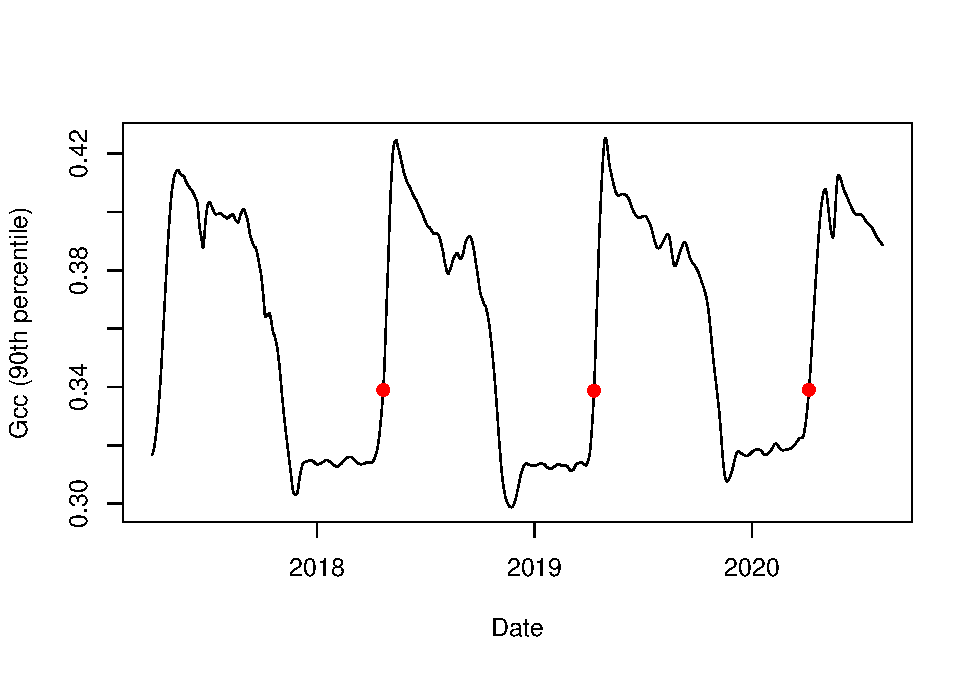
\includegraphics{phenology_example_files/figure-latex/plotting-1.pdf}

\end{document}
